\documentclass[12pt]{report}
\usepackage[utf8]{inputenc}
\usepackage{graphicx}
\usepackage{geometry}
\usepackage{titlesec}
\usepackage{lipsum} % This package generates filler text. Remove it in your actual document.
\usepackage[hidelinks]{hyperref}
\renewcommand{\thesection}{\arabic{section}}

% Set the page margins.
\geometry{a4paper, margin=1in}

% Set the section title spacing and format.
\titleformat{\section}
  {\normalfont\Large\bfseries}{\thesection}{1em}{}
\titlespacing*{\section}
  {0pt}{3.5ex plus 1ex minus .2ex}{2.3ex plus .2ex}

% Define custom commands for common elements.
\newcommand{\keyword}[1]{\textbf{#1}}
\newcommand{\characters}[1]{(\textit{min #1 characters})}

% Title Page
\title{EK: Rapor Format}
\author{Your Name}
\date{\today}

% Adjust secnumdepth to ensure sections are numbered
\setcounter{secnumdepth}{3} % Number sections, subsections, and subsubsections

% Adjust tocdepth to control the depth of the ToC
\setcounter{tocdepth}{3} % Include sections, subsections, and subsubsections in the ToC

\begin{document}

\maketitle

% Abstract
\begin{abstract}
The "Crypto Data Analysis and Education Platform" is designed to serve as a comprehensive nexus for learners, investors, and enthusiasts of the cryptocurrency world. This platform stands out by providing real-time market data, educational content, and tools necessary for users to make informed decisions in the fast-paced realm of cryptocurrencies. It aims to demystify the complexities of blockchain technology and crypto assets through a user-friendly interface that caters to both novices and seasoned traders. The educational component is akin to a digital academy, offering courses and materials that range from the fundamentals of blockchain to advanced trading strategies. The analysis feature empowers users with actionable insights into market trends and potential investments. With a focus on security and up-to-date information, the platform integrates various technological solutions, including microservices for scalability, WebSocket for real-time updates, and advanced encryption for data protection. This project stands at the intersection of educational technology and financial innovation, aspiring to enhance the cryptocurrency community's literacy and investment acumen.
\end{abstract}


\textbf{Key Words:} Cryptocurrency Education, Blockchain Technology, Market Analysis, Crypto Portfolio Management, Decentralized Finance (DeFi), Digital Currency Trends, Blockchain Data Visualization, Crypto Trading Strategies, Financial Technology (FinTech), Smart Contract Development, Cryptography and Security, Distributed Ledger Technology, Tokenomics and Cryptoassets, Crypto Exchange Integration, Real-Time Market Data, Crypto Investment Analysis, Blockchain for Education, Crypto Regulatory Compliance, Decentralized Applications (DApps), Cryptocurrency News and Events.


% Add table of contents
\tableofcontents
\renewcommand{\thechapter}{\arabic{chapter}}
\renewcommand{\thesection}{\arabic{section}}
\setcounter{secnumdepth}{3} % Number sections, subsections, and subsubsections
\setcounter{tocdepth}{3} % Include sections, subsections, and subsubsections in the ToC

\newpage

% Introduction
\section{Introduction \characters{5000}}
The rise of blockchain technology and cryptocurrencies has transformed the financial landscape, introducing novel ways of handling transactions and storing value. As these digital assets gain popularity, the need for education, reliable data analysis, and news dissemination becomes increasingly vital. The ``Crypto Data Analysis and Education Platform'' aims to address these needs by providing a comprehensive resource for both novices and seasoned crypto enthusiasts.

This platform is designed to bridge the gap between complex blockchain technology and the general public by demystifying crypto concepts and promoting an understanding of its fundamentals through educational resources. Users will have access to a variety of tools that assist in tracking market trends and managing personal crypto portfolios, ensuring they are well-equipped to make informed decisions.

Moreover, the platform will feature real-time updates and analytical insights into the fast-evolving world of cryptocurrencies. By integrating educational content with up-to-date market analysis, the platform seeks to empower users with knowledge and practical tools, making them adept at navigating the crypto market.

Additionally, the platform will include an extensive range of features such as an admin panel for content management, a blog editor akin to Notion, and an education platform reminiscent of Udemy. These features are designed to enhance user engagement and provide tailored educational experiences, making the platform a central hub for crypto learning and analysis.

In essence, the ``Crypto Data Analysis and Education Platform'' not only serves as a tool for personal portfolio management but also as a beacon of knowledge, contributing to the safety and accessibility of cryptocurrency investments. This project, by addressing the educational gap and providing analytical tools, aligns with the ongoing advancements in cryptocurrency technologies and the increasing global interest in digital currencies.


% Realistic Constraints and Conditions
\section{Realistic Constraints and Conditions}

\subsection{Sustainable Development Goal \characters{1000}}
The ``Crypto Data Analysis and Education Platform'' aligns with several United Nations Sustainable Development Goals (SDGs), notably SDG 4: Quality Education, SDG 9: Industry, Innovation and Infrastructure, and SDG 10: Reduced Inequalities. By providing accessible, high-quality educational resources on cryptocurrencies and blockchain technology, the platform contributes directly to SDG 4. It enhances the availability of quality education materials and lifelong learning opportunities for all, regardless of geographic location or economic status.

Innovatively, the platform utilizes cutting-edge technology to disseminate information and provide user-friendly tools for data analysis and portfolio management, aligning with SDG 9. This fosters innovation through the integration of advanced technologies in the educational landscape, promoting a robust infrastructure for learning and engagement in the crypto economy.

Furthermore, by democratizing access to information and financial tools, the platform addresses SDG 10, which aims to reduce inequality within and among countries. It provides equal opportunities for all users to gain financial literacy and participate in the growing digital economy, thereby helping to lessen income and opportunity disparities globally.

Through these contributions, the platform not only advances cryptocurrency education but also plays a pivotal role in promoting sustainable development by integrating educational outreach with technological innovation and inclusivity.

\subsection{Effects on Health, Environment and the Problems of the Age Reflected in the Field of Engineering \characters{1000}}
The ``Crypto Data Analysis and Education Platform'' intersects crucially with contemporary societal and environmental challenges, particularly those addressed in the field of engineering. While cryptocurrencies themselves are often criticized for their environmental impact, primarily due to the energy-intensive nature of mining activities, this platform contributes positively by promoting the adoption of more sustainable blockchain technologies such as proof-of-stake protocols, which require significantly less energy than the traditional proof-of-work systems.

Moreover, the platform encourages the development and use of blockchain applications that can improve public health systems, such as secure and transparent medical record management and supply chain oversight for pharmaceuticals. By integrating advanced data analysis tools, it facilitates more informed decisions that can lead to improved health outcomes and more efficient resource allocation in healthcare settings.

From an engineering perspective, the platform addresses modern problems by promoting technological literacy and accessibility. It provides tools and educational resources that demystify advanced engineering concepts related to blockchain and cryptocurrency technologies, making these topics accessible to a broader audience. This not only helps in reducing the digital divide but also empowers individuals with the knowledge to engage in discussions and activities that shape the future of technology.

Thus, the platform not only enhances understanding and adoption of blockchain technology but also contributes to environmental sustainability and public health through its educational and technological initiatives. These contributions reflect a comprehensive approach to tackling the pressing issues of our time through innovative engineering solutions.

\subsection{Legal Consequences \characters{1000}}
The deployment and operation of the ``Crypto Data Analysis and Education Platform'' entail a thorough navigation of complex legal landscapes, particularly concerning data privacy, cryptocurrency regulations, and intellectual property rights. In the realm of data privacy, adherence to regulations such as the General Data Protection Regulation (GDPR) in Europe and similar laws globally is imperative. The platform is committed to ensuring the confidentiality, integrity, and availability of user data, employing state-of-the-art security measures to protect personal information and transaction details.

Furthermore, as the platform deals with cryptocurrency data and provides tools for financial analysis and management, compliance with financial regulations is crucial. This includes observing the guidelines set by financial authorities regarding the reporting and transparency of cryptocurrency transactions to prevent money laundering and financial fraud. The platform ensures that all features comply with the legal standards of each jurisdiction in which it operates, adapting to ongoing changes in cryptocurrency legislation.

Additionally, the platform must consider intellectual property laws, especially concerning the content generated for educational purposes and the proprietary technology developed for data analysis and portfolio management. This involves securing copyrights for educational content and patents for unique technological innovations, where applicable, to protect the platform’s assets and intellectual contributions.

Navigating these legal requirements is not only necessary for compliance but also crucial in building trust with users and stakeholders. By adhering to these legal standards, the platform ensures its long-term viability and integrity in the highly scrutinized domain of cryptocurrency and blockchain technology.



Here's a comprehensive draft for the "Literature Analysis" section of your report based on a systematic review of the recent literature on cryptocurrency education platforms and blockchain technology's role in education.

\section{Literature Analysis \characters{8000}}
The advent of blockchain technology has sparked a significant interest across various sectors, including education, where it is seen as a potential driver for innovation and trust. A systematic literature review reveals that blockchain technology is increasingly incorporated in educational systems, emphasizing decentralized, secure, and transparent learning environments. This aligns with the objectives of the "Crypto Data Analysis and Education Platform" which seeks to integrate blockchain for educational purposes.

Recent studies highlight blockchain's role in enhancing trust and security in educational transactions, which is crucial for the authenticity of certifications and the management of educational records. Furthermore, the application of blockchain in education extends to facilitating lifelong learning opportunities and supporting decentralized education models. These aspects are particularly pertinent to the platform's goal of providing a comprehensive and trustworthy educational environment on cryptocurrencies and blockchain technology.

Cryptocurrency education platforms also benefit from blockchain's ability to offer transparent and verifiable content, which is essential in an era where the authenticity of educational material can be crucial for both learners and educators. The technology also supports innovative learning solutions that can adapt to the needs of a global audience, fostering a more inclusive educational landscape.

Moreover, the literature identifies a growing trend towards the integration of cryptocurrencies within educational frameworks, either as a subject of study or as a medium for facilitating transactions within educational ecosystems. This dual approach not only enhances understanding of digital currencies but also encourages the practical use of blockchain technology in everyday educational administrative operations.

The intersection of blockchain technology with educational needs highlights its potential to address several persistent challenges within the sector, including issues of access, verification, and cost-efficiency. By leveraging blockchain, educational platforms can provide more scalable and flexible learning solutions that are aligned with modern technological advancements.

In conclusion, the systematic review of literature underscores the significant potential and ongoing developments in utilizing blockchain technology within educational sectors. It provides a strong foundation for the proposed "Crypto Data Analysis and Education Platform," aligning with its core objectives of educational dissemination, transparency, and user empowerment in the cryptocurrency domain.

\section{Standards to be Used \characters{1000}}
The ``Crypto Data Analysis and Education Platform'' will adhere to a set of established standards to ensure the reliability, security, and effectiveness of its services. These standards include:

\textbf{ISO/IEC 27001:} This standard is crucial for information security management systems (ISMS), providing a systematic approach to managing sensitive company information so that it remains secure. It includes people, processes, and IT systems by applying a risk management process.

\textbf{WCAG 2.1:} The Web Content Accessibility Guidelines ensure that content is accessible to all users, including those with disabilities. This aligns with the platform's commitment to inclusivity.

\textbf{IEEE Standards:} Utilizing IEEE standards for software development and data interoperability ensures that the platform's technological solutions are robust and adhere to international guidelines for engineering quality.

\textbf{Open Badges 2.0:} For educational achievements, the platform will integrate Open Badges 2.0, a standard to recognize and verify learning achievements with digital badges issued by credible organizations.

\textbf{Cryptocurrency Security Standard (CCSS):} This is essential for ensuring that all systems that use cryptocurrencies adhere to security prerequisites that protect all information within a cryptocurrency system.

These standards are chosen to promote best practices in security, accessibility, education, and data handling, supporting the platform’s mission to provide a trustworthy and inclusive educational environment.

\section{Approaches, Techniques, and Technologies to be used \characters{6000}}
The development and operation of the ``Crypto Data Analysis and Education Platform'' encompass a variety of modern approaches, techniques, and technologies designed to create a robust, scalable, and user-friendly environment. The key aspects include:

\textbf{Microservices Architecture:} Utilizing a microservices architecture, particularly through NestJS, enables the platform to be highly scalable and maintainable. This architecture allows for the independent scaling of different parts of the application, which is essential for handling varying loads and introducing new features without downtime.

\textbf{React Native and Expo for Mobile Development:} These technologies allow for the development of cross-platform mobile applications that provide a native app experience. React Native and Expo are chosen for their ability to accelerate development and facilitate easier maintenance and updates across iOS and Android devices.

\textbf{Next.js for Web Frontend:} Leveraging Next.js enhances the platform's SEO, improves performance with server-side rendering, and provides a rich set of features for building interactive user interfaces. It supports static site generation and server-side rendering, crucial for content-heavy platforms like blogs and educational modules.

\textbf{GRPC for Inter-Service Communication:} GRPC is used for efficient, low-latency communication between microservices. It supports multiple programming languages, making it a versatile choice for a distributed system that requires a high-throughput and robust service-to-service communication protocol.

\textbf{Prisma as ORM:} Prisma is integrated to manage the platform’s data layer effectively. It provides a powerful query engine and type safety, which enhances the development speed and reliability of database operations.

\textbf{Redis for Caching and Pub/Sub:} Redis is employed to manage real-time data efficiently, crucial for features like live cryptocurrency price updates and notifications. Its use in caching responses reduces latency and load on the database.

\textbf{WebSocket for Real-Time Communication:} WebSocket is implemented to enable real-time bi-directional communication between clients and servers, essential for live data feeds and interactive user interfaces.

\textbf{TypeScript:} All components of the platform are developed using TypeScript, enhancing code quality and maintainability through strong typing and object-oriented features.

\textbf{CCXT for Cryptocurrency Exchange Data:} The CCXT library is integrated to connect with multiple cryptocurrency exchanges, providing users with extensive data and enabling complex trading strategies.

\textbf{E-Charts for Data Visualization:} E-Charts is utilized to render complex graphical data representations, crucial for visualizing market trends and cryptocurrency analytics effectively.

These approaches, techniques, and technologies are selected to ensure that the platform is secure, efficient, and capable of handling the specific needs of cryptocurrency enthusiasts and learners.

\section{Risk Management}
\begin{table}[h]
\centering
\begin{tabular}{|l|p{6cm}|p{5cm}|}
\hline
\textbf{WP-No} & \textbf{Risks}                                 & \textbf{Risk Management (Plan B)}          \\ \hline
WP1            & Incomplete requirements, technical debt         & Regular reviews, stakeholder consultations \\ \hline
WP2            & Integration issues, performance bottlenecks     & Prototyping, performance testing           \\ \hline
WP3            & Usability issues, browser compatibility         & Usability testing, cross-browser testing   \\ \hline
WP4            & Data migration errors, scalability concerns     & Data validation checks, scalability testing\\ \hline
WP5            & Insufficient test coverage, missed bugs         & Comprehensive test plans, continuous integration \\ \hline
WP6            & Downtime, deployment failures                  & Staging environment tests, rollback strategy \\ \hline
\end{tabular}
\caption{Risk Management Strategies}
\label{table:risk_managementand}
\end{table}

Effective risk management is pivotal in ensuring the successful delivery of the ``Crypto Data Analysis and Education Platform.'' Each work package (WP) within the project encapsulates a set of risks that could potentially impede progress. The identification of these risks and the development of mitigation strategies, referred to as Plan B, are critical components of our project management strategy.

\subsection{WP1: Requirements and Technical Debt}
Incomplete or misunderstood requirements can lead to technical debt that, if not managed properly, can cause significant delays in later project stages. Regular review sessions with stakeholders and iterative refinement of requirements are necessary to minimize this risk. The technical debt will be periodically reassessed to ensure that any incurred debt is identified early and addressed promptly.

\subsection{WP2: Integration and Performance}
As the platform integrates various microservices and third-party APIs, there may be risks related to system integration and performance bottlenecks. To counteract this, prototyping and performance testing will be conducted early and continuously throughout the development lifecycle. This proactive approach ensures performance standards are met and integration issues are resolved early.

\subsection{WP3: Usability and Browser Compatibility}
Usability is crucial for ensuring that the platform remains accessible and easy to navigate for all users. Similarly, browser compatibility issues can prevent users from accessing the platform across different devices. Usability testing, coupled with extensive cross-browser testing, will be conducted to ensure the platform provides a consistent user experience on all supported browsers.

\subsection{WP4: Data Migration and Scalability}
The platform's evolution may necessitate data migration, which poses risks related to data integrity and scalability. Data validation checks will be implemented to prevent errors during migration. Additionally, scalability testing will be conducted to ensure the platform can handle increased loads without degradation in performance.

\subsection{WP5: Test Coverage and Missed Bugs}
Insufficient test coverage and undetected bugs can undermine the platform's reliability. A comprehensive test plan, incorporating unit, integration, and system tests, will be established. Continuous integration practices will be employed to ensure that tests are run automatically and frequently, allowing for the early detection of faults.

\subsection{WP6: Downtime and Deployment Failures}
Operational risks such as downtime and deployment failures can affect the platform's availability. Staging environment tests, along with a well-defined rollback strategy, will be employed to minimize service interruptions and ensure smooth deployment cycles.

Each mitigation strategy will be regularly reviewed and updated as the project progresses to respond to new risks and challenges that may emerge. By maintaining a dynamic and responsive risk management plan, the project team aims to deliver the ``Crypto Data Analysis and Education Platform'' efficiently and effectively, minimizing disruptions and maximizing quality.


\section{Project Schedule and Task Sharing}
A comprehensive project schedule and task sharing plan is critical to the timely and successful delivery of the ``Crypto Data Analysis and Education Platform.'' This section outlines the division of work packages (WPs), the assignments of tasks to staff members, the time periods allocated for each WP, and the criteria for their successful completion.

\subsection{WP1: System Architecture}
The project commences with the development of a robust system architecture. This initial phase involves defining and documenting the technical and architectural specifications that will guide subsequent development efforts.

\subsection{WP2: Backend Development}
Following the establishment of the system architecture, backend development begins. This stage focuses on implementing REST API endpoints, ensuring a solid foundation for the platform's functionality.

\subsection{WP3: Frontend Development}
Concurrently with backend development, the frontend team will work on translating design specifications into a functional user interface. This phase is critical for engaging users with a seamless experience.

\subsection{WP4: Database Integration}
Database design and integration occur alongside front and backend development. This WP ensures that data storage and retrieval processes are optimized and scalable.

\subsection{WP5: Testing \& QA}
Quality assurance and testing are ongoing processes that ramp up significantly after primary development. All tests must pass with greater than 90\% coverage, guaranteeing the reliability and stability of the platform.

\subsection{WP6: Deployment}
The final phase involves deploying the application to the production server. This WP includes final stress testing and the preparation of roll-back strategies to ensure a smooth launch.

Each WP is assigned a specific time frame, and the assigned staff is responsible for meeting the outlined success criteria within the allocated period. This structured approach ensures clear responsibilities and deadlines, thereby facilitating efficient project management and execution.

\begin{table}[h]
\centering
\begin{tabular}{|l|l|l|p{2cm}|p{4cm}|}
\hline
\textbf{WP-No} & \textbf{Work Package Name} & \textbf{Assigned Staff} & \textbf{Time Period} & \textbf{Success Criteria} \\ \hline
WP1            & System Architecture        & Emre YILDIZ             & 01-02                & Architecture defined \& documented \\ \hline
WP2            & Backend Development        & Emre YILDIZ             & 02-04                & REST API endpoints implemented \\ \hline
WP3            & Frontend Development       & Emre YILDIZ             & 03-05                & User interface matches design specs \\ \hline
WP4            & Database Integration       & Emre YILDIZ             & 04-06                & Database schema designed \& integrated \\ \hline
WP5            & Testing \& QA              & Emre YILDIZ             & 06-07                & All tests pass with $>$ 90\% coverage \\ \hline
WP6            & Deployment                 & Emre YILDIZ             & 07-08                & Application deployed to production server \\ \hline
\end{tabular}
\caption{Project Scheduling and Tasks Sharing}
\label{table:project_schedule}
\end{table}



\section{System Requirements Analysis}

\subsection{Use Case Model \characters{3000}}
The Use Case Model for the ``Crypto Data Analysis \& Education Platform'' serves as a blueprint for defining the system interactions from the perspective of end-users. It encapsulates the comprehensive functionalities of the platform and the real-world scenarios in which these functionalities are employed by various actors.

\textbf{Actors:} The primary actors include \textit{Registered Users}, \textit{Guest Visitors}, \textit{System Administrators}, and \textit{Content Creators}. Registered Users have access to personalized features like portfolio management and market trend notifications. Guest Visitors can access public educational resources and news. System Administrators manage platform operations, and Content Creators publish educational content and analyses.

\textbf{Use Cases:}
\begin{enumerate}
    \item \textit{Portfolio Management:} Registered Users can create and manage a cryptocurrency portfolio, tracking real-time asset performance and receiving customized advice.
    \item \textit{Educational Resource Access:} Both Registered Users and Guest Visitors can access a wide range of educational materials, ranging from introductory articles to advanced tutorials.
    \item \textit{Market Analysis:} Registered Users benefit from in-depth market analyses, leveraging historical data and predictive models to gain investment insights.
    \item \textit{Content Publication:} Content Creators publish blog posts, analysis papers, and news articles, which are then vetted by System Administrators for quality assurance before release.
    \item \textit{Real-Time Notifications:} Registered Users opt into notifications for market movements, news updates, and educational opportunities relevant to their interests and portfolio holdings.
\end{enumerate}

Each use case is structured to facilitate a particular set of interactions with the platform, providing a clear path for meeting the diverse needs of the platform's user base. The use cases are designed to be modular and scalable, allowing for the addition of new features as the platform evolves.

This Use Case Model is pivotal for identifying the system requirements that will guide the design and development of the ``Crypto Data Analysis \& Education Platform.'' It forms the foundation for creating a user-centric, intuitive, and comprehensive educational platform in the crypto space.


\subsection{Object Model \characters{3000}}
The Object Model for the ``Crypto Data Analysis and Education Platform'' articulates the static structure of the platform by detailing the objects, their attributes, operations, and the relationships among them. It is a blueprint that defines the data structure and represents the domain of the problem the platform addresses.

\textbf{Key Objects:}
\begin{itemize}
    \item \textit{User:} Represents both registered and guest users with attributes such as \texttt{userID}, \texttt{username}, \texttt{portfolio}, and operations like \texttt{login()}, \texttt{logout()}, \texttt{viewResources()}.
    \item \textit{Content:} Encapsulates all educational and news-related material with attributes like \texttt{contentID}, \texttt{title}, \texttt{body}, and operations including \texttt{publish()}, \texttt{update()}, \texttt{archive()}.
    \item \textit{Portfolio:} Maintains user's cryptocurrency holdings with attributes such as \texttt{portfolioID}, \texttt{assets}, and operations like \texttt{addAsset()}, \texttt{removeAsset()}, \texttt{getPerformance()}.
    \item \textit{MarketData:} Contains real-time and historical market information with attributes like \texttt{dataID}, \texttt{price}, \texttt{volume}, and operations such as \texttt{updatePrice()}, \texttt{getTrends()}, \texttt{calculateIndicators()}.
\end{itemize}

\textbf{Relationships:}
\begin{itemize}
    \item A \textit{User} can have one or many \textit{Portfolios}, implying a one-to-many relationship between \textit{User} and \textit{Portfolio}.
    \item \textit{Content} is created by \textit{Content Creators}, indicating a one-to-many relationship from \textit{Content Creators} to \textit{Content}.
    \item \textit{MarketData} is associated with multiple \textit{Portfolios} to provide market insights, representing a many-to-many relationship.
\end{itemize}

\textbf{Classes:}
Classes such as \texttt{User}, \texttt{Content}, \texttt{Portfolio}, and \texttt{MarketData} are designed with encapsulation to maintain the integrity of the data and provide the necessary functionalities. Each class includes methods for the creation, manipulation, and presentation of its data, ensuring that the system's operations align with user actions and intentions.

This Object Model serves as the fundamental design for the platform's backend structure, ensuring data consistency and facilitating the platform's core functionality. It is the architectural framework upon which dynamic processes and user interactions are built, providing a systematic approach to developing the platform's software components.
\clearpage % Ensures the image appears on a new page
\begin{figure}[p] % 'p' places the figure on a page containing only floats, such as tables and figures.
\centering % Centers the image
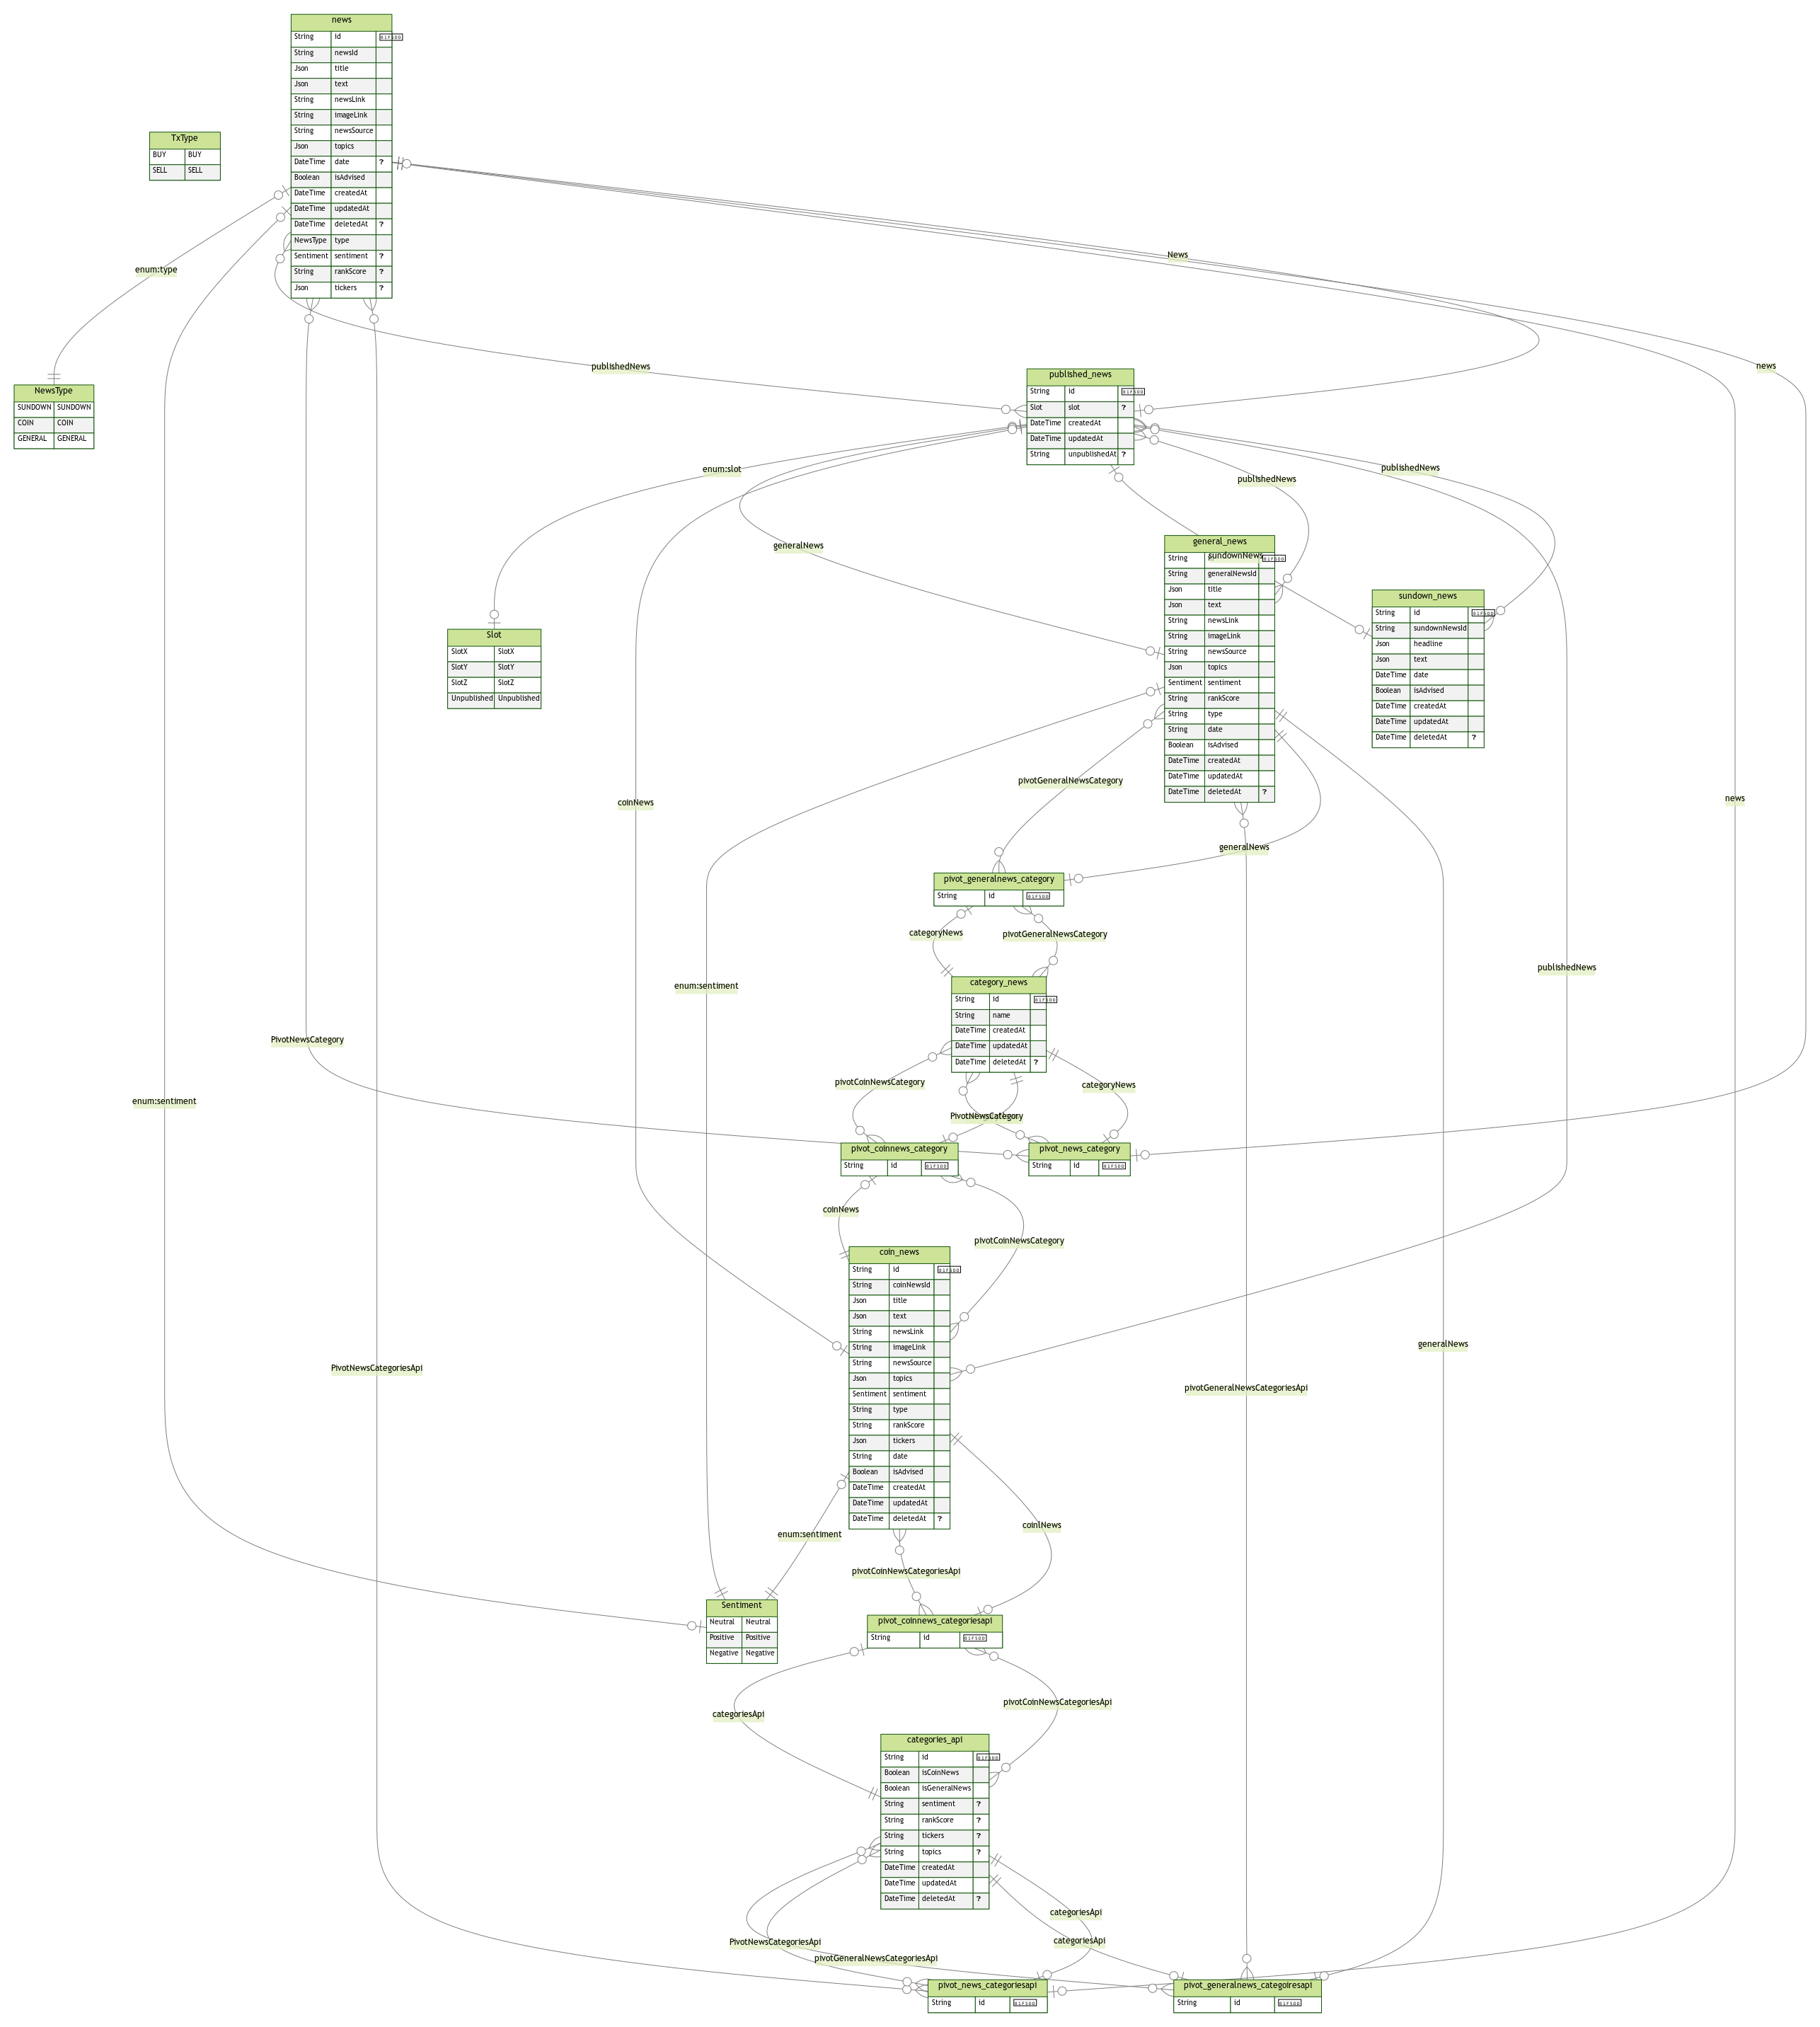
\includegraphics[width=\textwidth,height=\textheight,keepaspectratio]{ERD.png} % Adjusts the size to fit the page
\caption{Entity Relationship Diagram of the System} % Optional: add a caption
\label{fig:er_diagram} % Optional: label for referencing the figure
\end{figure}
\clearpage % Ensures any following content appears on a new page

\clearpage % Ensures the image appears on a new page
\begin{figure}[p] % 'p' places the figure on a page containing only floats, such as tables and figures.
\centering % Centers the image
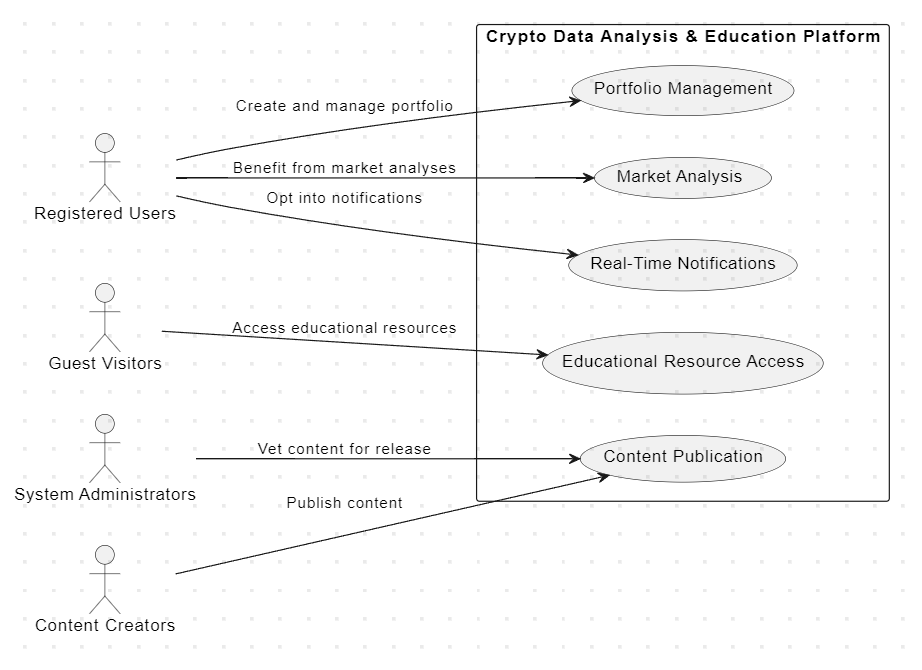
\includegraphics[width=\textwidth,height=\textheight,keepaspectratio]{use-case.png} % Adjusts the size to fit the page
\caption{Use Case Diagram of the System} % Optional: add a caption
\label{fig:er_diagram} % Optional: label for referencing the figure
\end{figure}
\clearpage % Ensures any following content appears on a new page
\begin{thebibliography}{9}
\bibitem{latexcompanion} 
Michel Goossens, Frank Mittelbach, and Alexander Samarin. 
\textit{The \LaTeX\ Companion}. 
Addison-Wesley, Reading, Massachusetts, 1993.
 
\bibitem{einstein} 
Albert Einstein. 
\textit{Zur Elektrodynamik bewegter K{\"o}rper}. (German) 
[\textit{On the Electrodynamics of Moving Bodies}]. 
Annalen der Physik, 322(10):891–921, 1905.
 
\bibitem{knuthwebsite} 
Knuth: Computers and Typesetting,
\\\texttt{http://www-cs-faculty.stanford.edu/\~{}uno/abcde.html}
\end{thebibliography}


\section{Choose Interdisciplinary Domain of Study}
[8.Decent Work and Economic Growth]

\end{document}
